\section{Introduction}
\todo{ref ?Kandel -  no I have the references for size and complexity and therefore connections and complexity will continue looking as finish things off this remains a todo if not just cite the SG paper referring to the neuronal hypothesis}

\section{Chapter Cnetrality}

\cite{newman2003social}
\cite{vasques2020transitivity}


\subsection{Biomedical significance}
\textcolor{red}{this is about ones that don't quite fit in}
A number of studies have looked at induced subnetworks such that the subnetwork contains a high proportion of genes with a high significance score related to the trait in question and reported centrality values. Although protein networks are included in such studies eg Liu they are similar to the WGCNA methods in treating the topology as a result of the experiment rather than comparing the features of the network topology to the results of experiment. I have not adopted this strategy and they are summarised in an overview by Nikolayeva\cite{nikolayeva2018network}.


\subsection{Centrality measures and pLI}

The higher centrality measures are the higher is the probability of loss of function intolerance. The relationship is  moderately strong for all centrality measures other than transitivity see table~\ref{tab:Correlation of Centrality measures with probability of loss of function intolerance (pLI) gnomad.}
% latex table generated in R 3.6.3 by xtable 1.8-4 package
% Sun Oct 18 17:25:49 2020
\begin{table}[ht]
\centering
\begin{tabular}{rrrr}
  \hline
 & S & rho & p \\ 
  \hline
degree & $5.14 \times 10^{9}$ & 0.225 & $2.37 \times 10^{-40}$ \\ 
  betweenness\_centrality & $5.29 \times 10^{9}$ & 0.202 & $1.29 \times 10^{-32}$ \\ 
  eigenvector & $5.21 \times 10^{9}$ & 0.213 & $2.59 \times 10^{-36}$ \\ 
  closeness & $5.14 \times 10^{9}$ & 0.225 & $2.20 \times 10^{-40}$ \\ 
  transitivityNA & $4.54 \times 10^{9}$ & 0.097 & $5.66 \times 10^{-8}$ \\ 
  kcoreness & $5.10 \times 10^{9}$ & 0.231 & $1.95 \times 10^{-42}$ \\ 
   \hline
\end{tabular}
\caption{Correlation of Centrality measures with probability of loss of function intolerance (pLI) gnomad.\url{source('~/RProjects/db_essential_genes/R/gnomad/correlation/correlation_gnomad/pLI_graph/cor_pLI_and_graph.R')}} 
\label{tab:Correlation of Centrality measures with probability of loss of function intolerance (pLI) gnomad.}
\end{table}
Mouse phenotype abnormal cell proliferation.

Disgennet2r tables moved to section~\ref{sec:disgennet2r tables}
\paragraph{Move}
This is the metadata reference \cite{newman2016structure}

\subsection{Degree Others}
Human phenotype number two is fronto temporal dementia, also includes abnormal emotion in table~\ref{tab:ToppGENE Human Phenotype. 90 centile cwpsp.txtp = p value; q FDR B H = q adjusted significance level False Discovery Rate using Benjamini and Hochberg adjustment; n= n genes annotated in test group; n PSP= n genes annotated in PSP. n significant in category 131}.
\section{Results Induced Subgraph: Association between significant vertices}
\todo[inline]{this goes with assortativity because it is about connections}
Do there tend to be edges between significant vertices? Do the vertices representing genes of genome wide significance form an induced subgraph that is connected?



The subgraph of significant genes is the graph formed by nodes defined as showing significant association with intelligence or educational attainment in the cohort studies and is induced upon the PSP network. The results are shown in table~\ref{tab:Largest connected component significant genes}

\begin{table}[ht]
\centering
\begin{adjustbox}{width=\textwidth}
\setlength{\extrarowheight}{2pt}
\begin{tabular}{rrrrrrrrrrrr}
  \toprule
 & $n$ in PSP & total genes & LCC & S\textsubscript{Min.} & S\textsubscript{Median} & S\textsubscript{Mean} & S\textsubscript{Max.} & $\frac{S>=LCC}{n}$ & $\frac{S=LCC}{n}$ & $\frac{S<LCC}{n}$ & $\frac{LCC}{\mu}$ \\ 
  \midrule
Int\textsubscript{R}  & 16 & 47 & 1 & 1 & 1 & 2 & 8 & 1.000 & 0.604 & 0.000 & 0.647 \\ 
  Ed\textsubscript{R}  & 25 & 99 & 1 & 1 & 2 & 2 & 13 & 1.000 & 0.310 & 0.000 & 0.452 \\ 
   Int\textsubscript{D} & 51 & 196 & 2 & 1 & 4 & 5 & 28 & 0.984 & 0.207 & 0.016 & 0.401 \\ 
  Ed\textsubscript{D}  & 58 & 235 & 3 & 1 & 5 & 6 & 28 & 0.842 & 0.188 & 0.158 & 0.503 \\ 
   \bottomrule
\end{tabular}
\end{adjustbox}
\caption[Largest connected component of significant genes]{Largest connected component significant genes. Where $LCC$ is largest connected component, $S$ is the vector of the Monte Carlo empirical sampling distribution for the largest connected component ($n$ iterations = 10,000), $S>LLC$ number of samples where the random LCC was greater than the study LCC. In general the largest connected component formed from genes that were genome wide significant in studies of educational attainment or intelligence were less than those of randomly selected vertices of the same size but there were still a significant number of samples equal to or less than the number of connected components.NB a LCC of one means that the graph is completely disconnected unless the size of the vertex set the subgraph is induced on is one. 
\tiny\url{source('~/RProjects/chapter3/R/mouse_ltp/test_study_connected_component_table_iterate.R')}}
\label{tab:Largest connected component significant genes}
\end{table}

The induced subgraph (See methods section~\ref{sec:method_induced_subgraph})\footnote{The graph with vertex set equal to a subset of the vertex set and the edge set equal to all edges in the graph that connect two members of the vertex subset} of significant genes for Intelligence\textsubscript{Replication} is 16 vertices no edges. Simulation mean 0.60 sd 0.94 N iterations = 1000.

For Education\textsubscript{Replication} it is 25 vertices no edges (simulation mean 1.51 sd 1.69). 

For Intelligence ED  \textsubscript{Discovery} it is 58 vertices with 4 edges. (Components one 2, one 3).  Simulation mean 8.78 sd 5.13.

For Education INT \textsubscript{Discovery} it is 51 vertices with 2 edges. 2 components of size 2.  Simulation mean 6.3 SD 4.1.

Simulation of joint results out of 1000, 100 trials (i.e. there are 1000 random subgraphs made of the same number of vertices as each study. For these we calculate
Min. 1st Qu.  Median    Mean 3rd Qu.    Max. 
   1.00    4.00    6.00    5.98    8.00   14.00 
   
   max = 14/1000 = 0.014
   mean = 0.006 of getting this number of edges or fewer in 4 samples of random subgraphs e.g.(number of times subgraph is 0 and next is 0 or less and next is 4 or less and next is 51 or less given actual frequency 0,0,4,2 and number of samples 16,25,58,51.
   
 \textcolor{red}{Need to redo I am getting confused}

UKBBEd

Number in PSP: 58 
Size of input: 235 
Largest component 3
Largest resampling component 32
Less than largest connected component 0.8514 
Greater than or equal to largest connected component 0.1486

% \begin{table}[ht]
% \centering
% \begin{adjustbox}{width=\textwidth}
% \begin{tabular}{rrrrrrrrrrrr}
%   \toprule
%  & num\_in\_PSP & total\_genes & largest\_component & Min. & Median & Mean & Max. & prop\_gt\_lcc & prop\_eq\_lcc & prop\_lt\_lcc & lcc\_to\_mean \\ 
%   \midrule
% ctg  & 16 & 47 & 1 & 1 & 1 & 2 & 8.000 & 1 & 0.604 & 0.000 & 0.647 \\ 
%   ea2  & 25 & 99 & 1 & 1 & 2 & 2 & 13.000 & 1 & 0.310 & 0.000 & 0.452 \\ 
%   ukbbint  & 51 & 196 & 2 & 1 & 4 & 5 & 28.000 & 1 & 0.207 & 0.016 & 0.401 \\ 
%   ukbbed  & 58 & 235 & 3 & 1 & 5 & 6 & 28.000 & 1 & 0.188 & 0.158 & 0.503 \\ 
%   \bottomrule
% \end{tabular}
% \end{adjustbox}
% \end{table}


% latex table generated in R 3.6.3 by xtable 1.8-4 package
% Mon Mar 15 14:30:04 2021

34.3\% less than or equal to size of largest connected component = 3

\begin{figure}
    \centering
    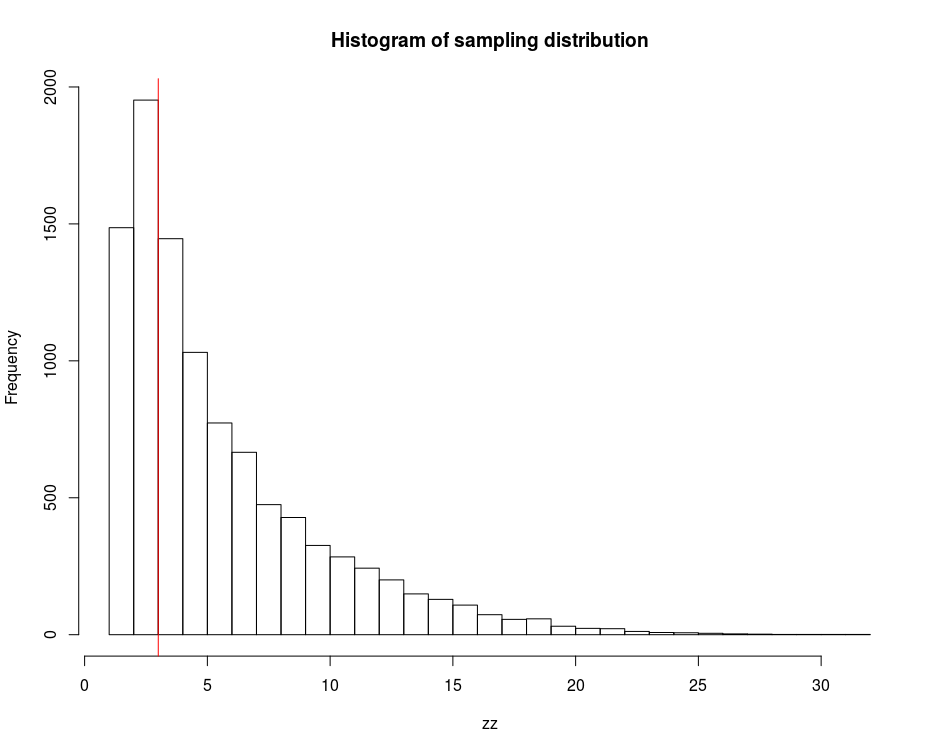
\includegraphics[width=\textwidth]{images/chapter3/connected_components/Rplot_ukbbed.png}
    \caption{Histogram of resampling of size of largest connected component n=58 in PSP UKBB Ed. 34.8\% less than or equal to 3. code \url{source('~/RProjects/chapter3/R/mouse_ltp/test_ukbbed_connected_component.R')}}
    \label{fig:my_label}
\end{figure}

 \subsubsection{Largest connected component and murine LTP}

Calculated the alrgest connect component induced by murine terms. 255 genes (should be 258 redo just need the more up to date data) are found in MP0002207 - abnormal long term potentiation. 140 of these are in the PSP. The largest connected component was 75 genes (140 nodes 125 edges in induced subgraph) 60 components largest 75. 

Resampling random samples of size 10000, 1 tailed t 0.0025

max 85.See figure~\ref{fig:histogram mouse ltp}

\begin{figure}
    \centering
    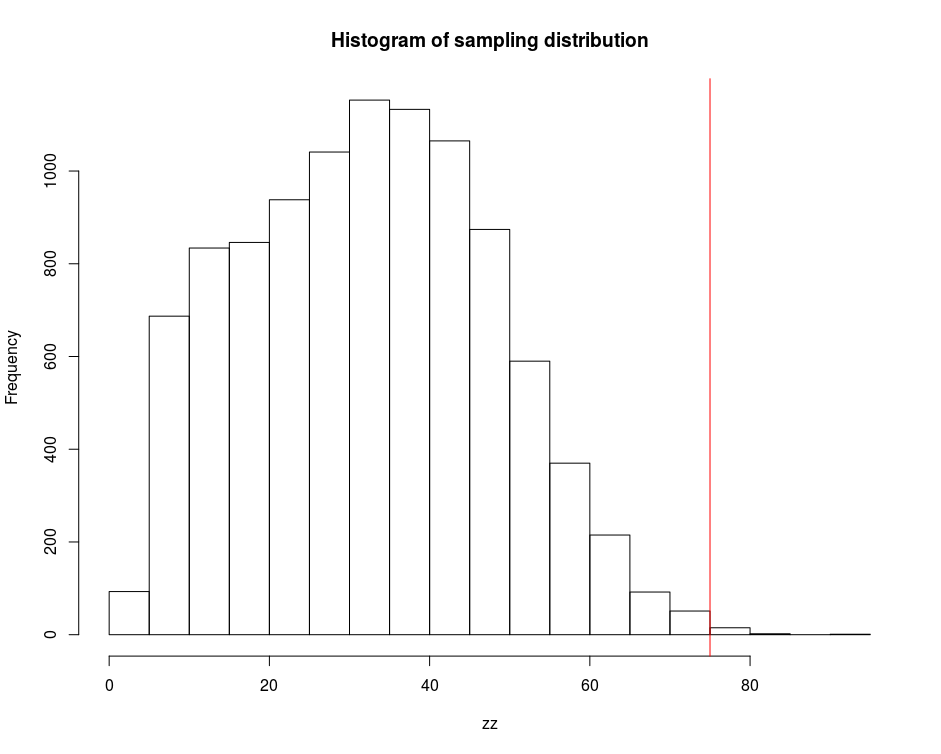
\includegraphics[width=\textwidth]{images/chapter3/connected_components/Rplot_mouse_abnormal_ltp_histogram_MP0002207.png}
    \caption{Histogram of resampling of size of largest connected component n=140 in PSP. Red line is size of mouse abnormal LTP 140 nodes in PSP. Largest component 75 Code\url{ source('~/RProjects/chapter3/R/mouse_ltp/test_murineLTP_connected_component.R')}}
    \label{fig:histogram mouse ltp}
\end{figure}


\section{Community detection benchmarks}

The block stochastic model provides generates with a Poisson distribution different to many real world networks (section~\ref{sec:stochastic block model}).

\subsection{LFR modularity}
\begin{table}[]
    \centering
    \begin{tabular}{ll}
    \toprule
    Method & modularity \\
    \midrule
        louvain & 0.432 (same) \\
infomap & 0.432   check\\
 greedy & 0.368 check\\
igraph eigenvector & 0.187\\
label propagation (10000) & 0.424 \\
walk trap  & 0.423 \\
sg1  & 0.433 \\
sg2 & 0.429 \\
sg5 & 0.379 \\
 spectral & 0.392\\
SBM & 0.189  \\
\bottomrule
         
    \end{tabular}
    \caption{Modularity for the LFR 3457 40617 graph. This is replicated current ipynb. Ref for Q greater than gt \cite{danon2006effect} }
    \tiny\url{g1 = nx.generators.LFR_benchmark_graph(n=graph_n,tau1= 2.51,tau2 = 1.5,mu= 0.375,min_degree=1 (commented out),average_degree=17,max_degree= 405, min_community= 15,max_community= 1000,seed=seed)} seed=1
    \tiny Red machine
    \tiny\url{/home/grant/Projects_/Python/src/LFR_networkx_to_igraph.ipynb}
    \label{tab:modularity for the LFR 3457 40617 graph}
\end{table}

\subsection{LFR q and mu plot}

\begin{figure}
    \centering
    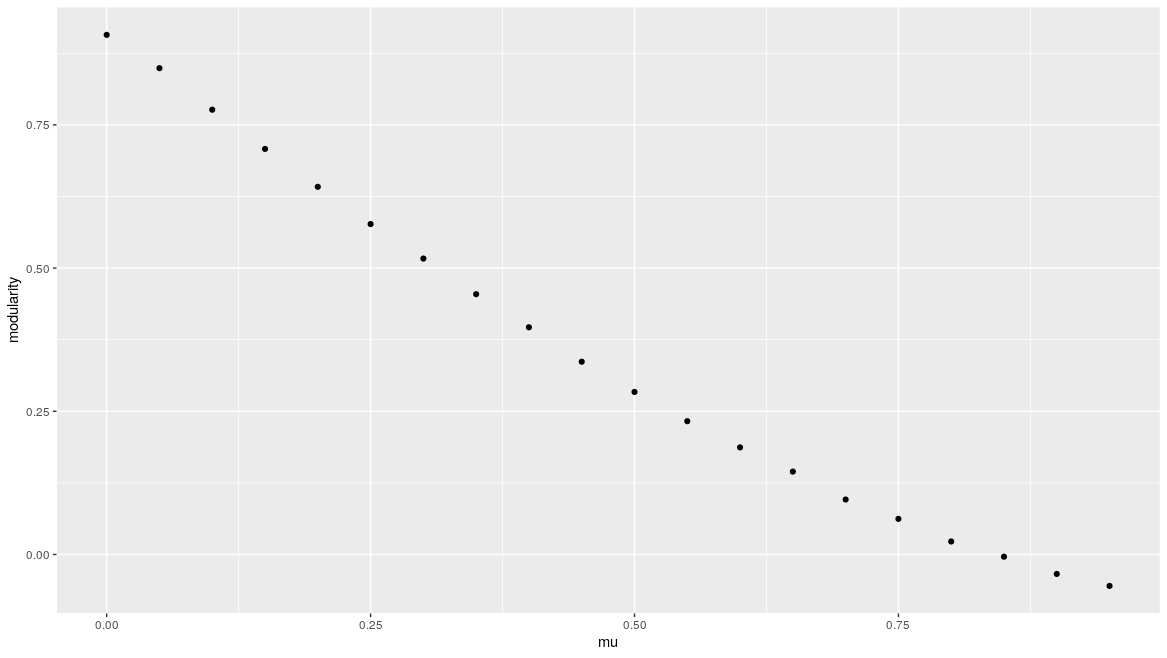
\includegraphics[width=0.9\textwidth]{images/Rplot_modularity_and_mu_series.png}
    \caption{Plot of modularity with parameter $mu$ in LFR benchmark. Source \url{source('~/RProjects/fortunato/R/plot_modularity_and_mu.R')}}
    \label{fig:modularity_and_mu}
\end{figure}

\section{Moved}
\subsection{Changed format tables Louvain}
\begin{table}[ht]
\centering
\begin{tabular}{rlrrrrrr}
  \hline
 & SET & NGENES & BETA & BETA\_STD & SE & Intelligence Discovery & Intelligence Replication \\ 
  \hline
2 & 2::: & 334 & 0.09 & 0.01 & 0.05 & 0.0407 & 0.1916 \\ 
  3 & 3::: & 510 & 0.10 & 0.02 & 0.04 & 0.0075 & 0.1006 \\ 
  7 & 7::: & 144 & 0.26 & 0.02 & 0.08 & 0.0012 & 0.0026 \\ 
  12 & 12::: & 21 & 0.63 & 0.02 & 0.21 & 0.0014 & 0.1628 \\ 
   \hline
\end{tabular}
\caption{Louvain clustering PSP Intelligence cohorts}
\label{tab:Louvain clustering intelligence}
\end{table}

% latex table generated in R 3.6.1 by xtable 1.8-4 package
% Sat Mar 28 15:49:04 2020
\begin{table}[ht]
\centering
\begin{tabular}{rlrrrrrr}
  \hline
 & SET & NGENES & BETA & BETA\_STD & SE & P & P\_EA2 \\ 
  \hline
2 & 2::: & 334 & 0.13 & 0.02 & 0.05 & 0.0071 & 0.0568 \\ 
  5 & 5::: & 112 & 0.23 & 0.02 & 0.09 & 0.0063 & 0.3478 \\ 
  7 & 7::: & 144 & 0.19 & 0.02 & 0.09 & 0.0146 & 0.4750 \\ 
   \hline
\end{tabular}
\caption{Louvain clustering PSP Education cohorts}
\label{tab:Louvain clustering education}
\end{table}


\subsection{Discussion}
\subsubsection{Extra discussion}

I have not included the Weibull as it seems implausible

The number of different factors that affect assortativity are going to play a role in any probabilistic model of a graph and in community formation

Note all report assortativity for example with random estimate

Generating mechanism of the lognormal is multiplication of random vvariables and is more common as dimensions increase above one dimension \cite{} ?discussion \cite{koch1966logarithm}
\cite{limpert2001log}

$C_k$ correlation misleading if not taken with $x_{min}$ like method

\textcolor{red}{The literature MOVE TO DISCUSSION} records a decrease in the average value of the clustering coefficient with increasing $k$. This has been done mostly for large networks such as the internet \cite{newman2018networks} p 335.
This relationship between $k$ and the transitivity $C$ therefore probably holds true in large networks (such as the internet where the studies were performed) where the number of nodes of low degree is dominated by the number of high degree (in this case $>=5$ nodes). 

\subsubsection{Assortativity and essential genes}
\label{sec:Assortativity and essential genes}
Latest 

assortativity nominal 0.0355
code\url{source('~/RProjects/db_essential_genes/R/get_essential_genes/assortativity_essential_genes.R')}

\subsubsection{Essential gene conclusion}
PSP genes are more likely to be essential. Essential genes are of higher degree than non essential genes. There is a very weak assortativity for essential genes. 

\todo{DONE Degree etc for essential genes}
\todo{Essential genes enrichment vs non essential PSP add to community detection section}
\todo{Essential gene count for significant genes vs psp genes}



\section{Chapter community detection}

\subsection{Removed from SBM benchmark}

For groups (Graph) \todo{labels} For groups (graph) \footnote{\url{source('~/RProjects/group_sizes/R/sbm_benchmark/graph/graph_performance_multi.R')}}

For nmi with ground truth Louvain\footnote{\url{source('~/RProjects/group_sizes/R/sbm_benchmark/graph/graph_performance.R')}}

The points here is that there is a dramatic deterioration in nmi for infomap (from perfect at 1 to 0) in figure~\ref{fig:my_nice_infomap} compared to figure~\ref{fig:my_sbmlouvain_nmi}. (what we are interested in here is points at which performance breaks down as infomap does very well on a lot of standard benchmarks)
\footnote{Source \url{source('~/RProjects/group_sizes/R/sbm_benchmark/graph/graph_performance.R')}}
\subsection{MAGMA methods from paper}
\begin{figure}
    \centering
    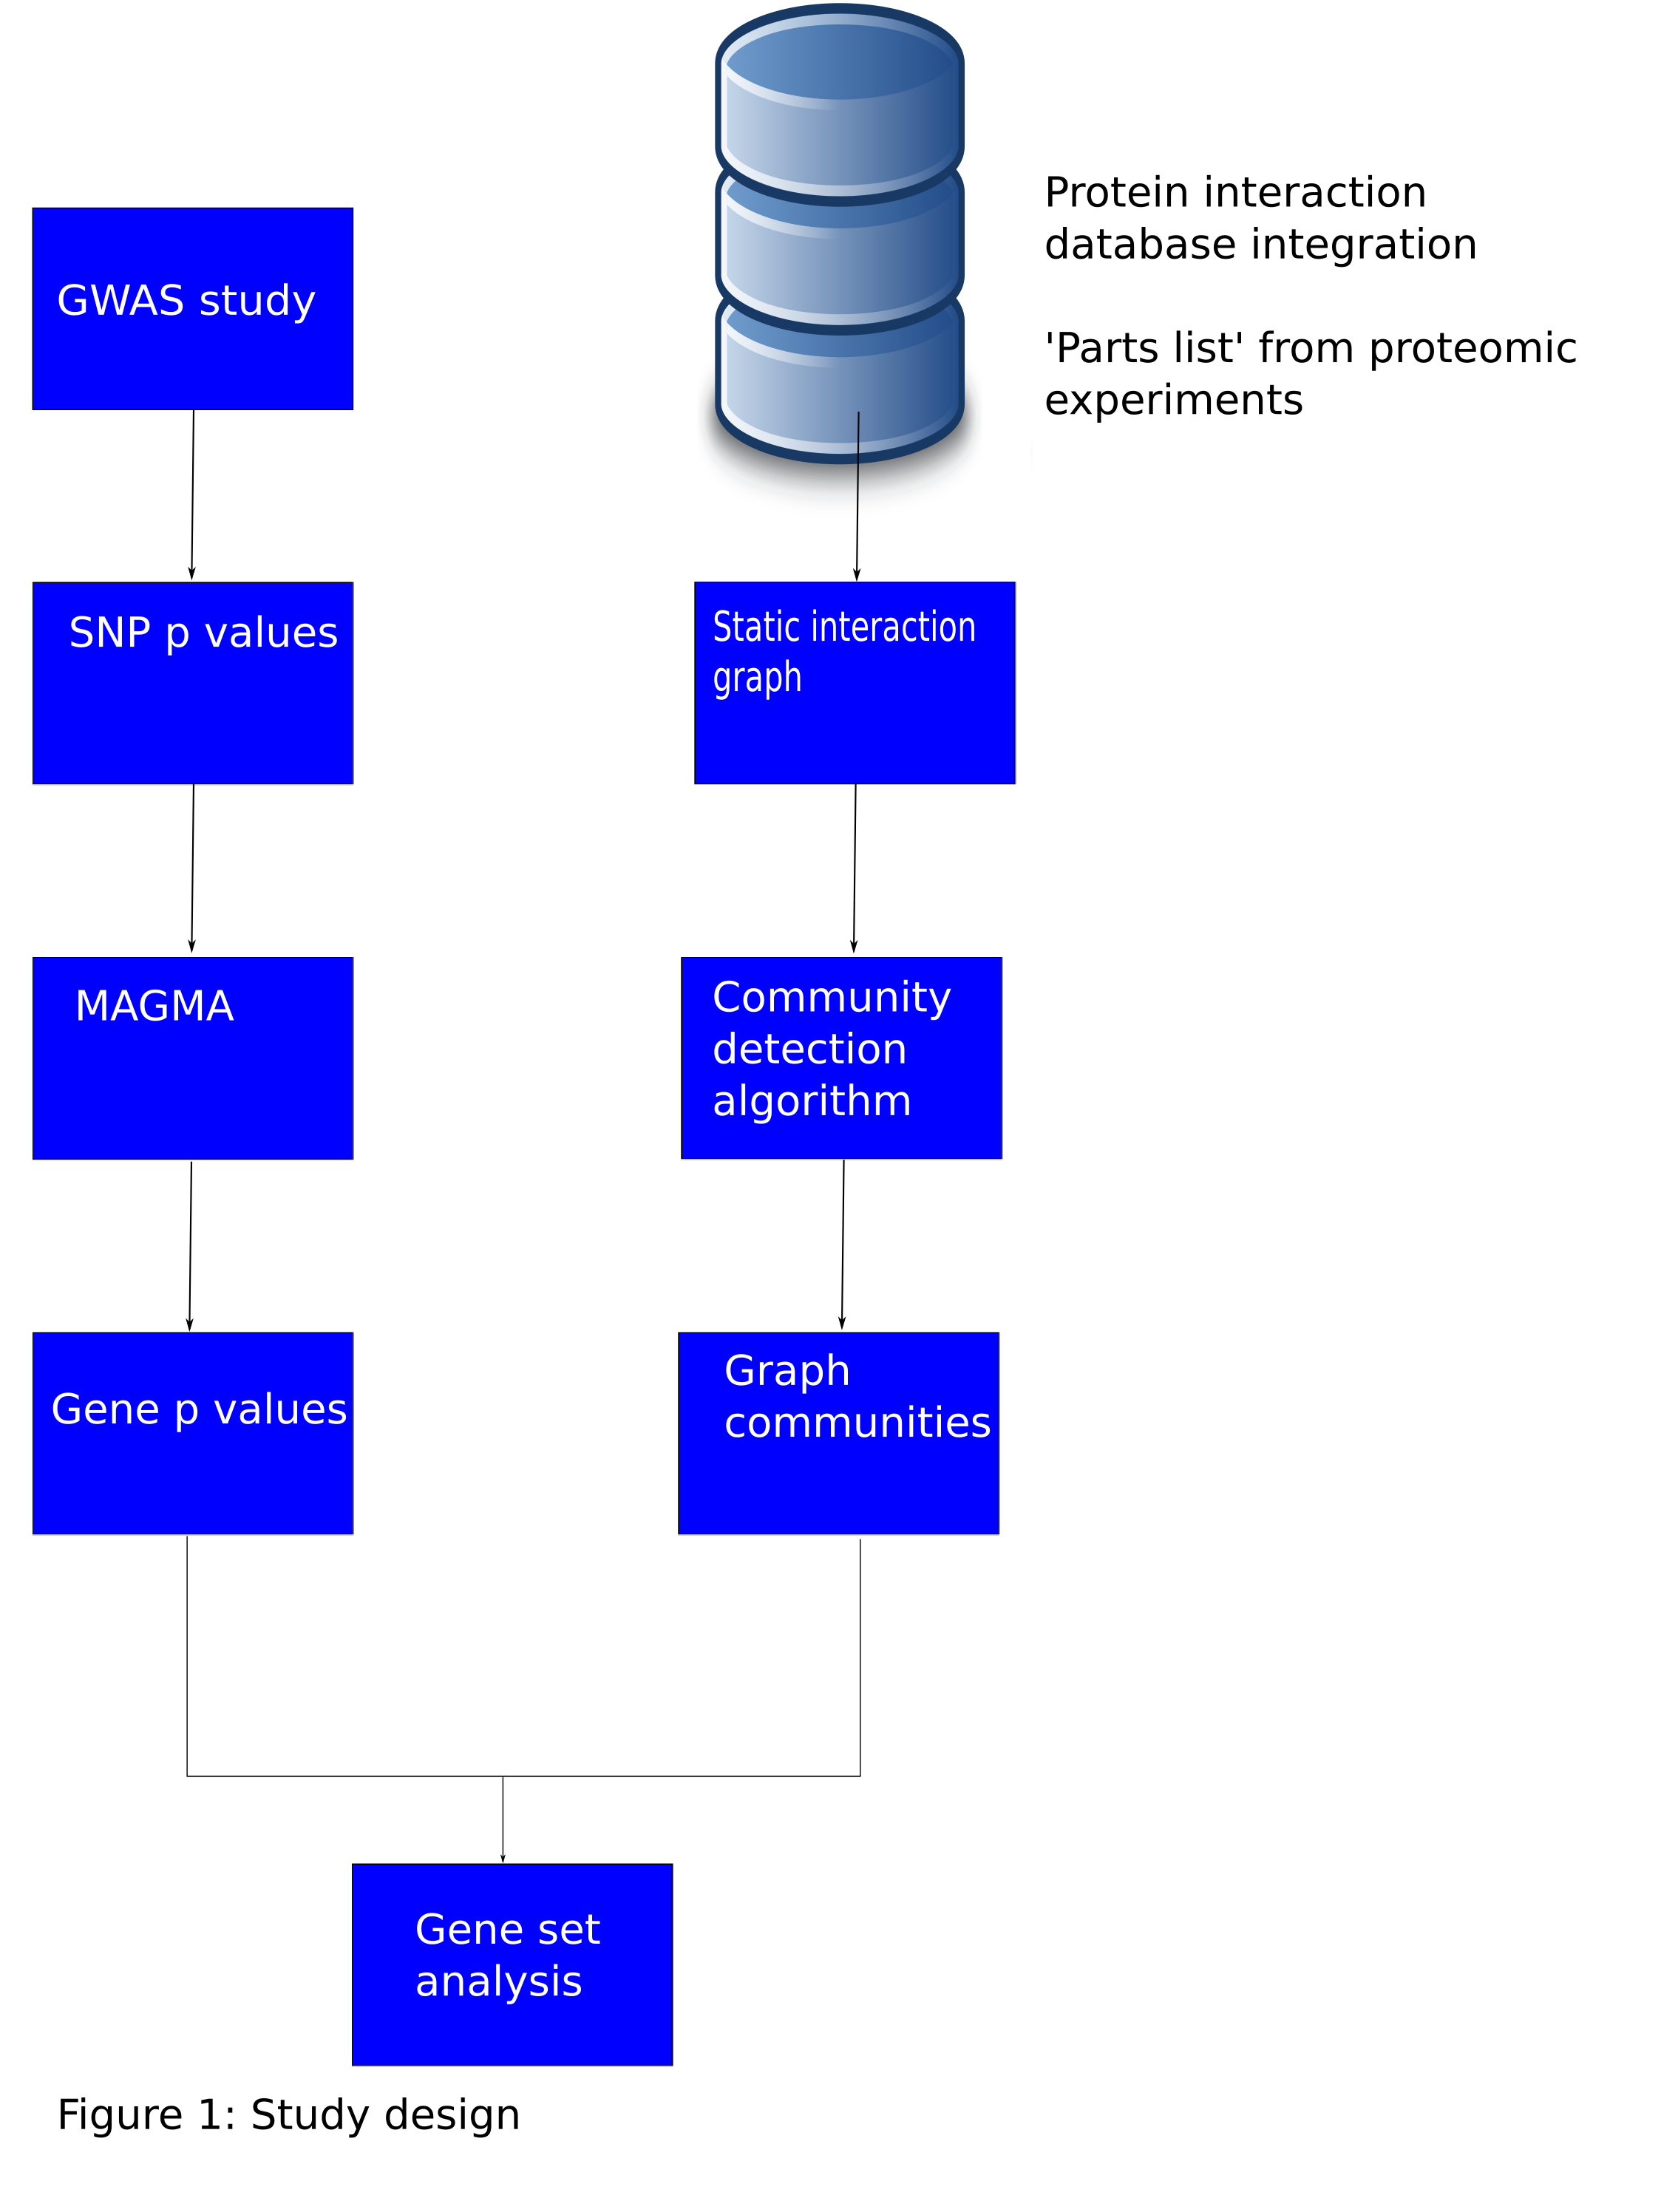
\includegraphics[width=\textwidth]{images/study_design.png}  
    \caption{Study design for community detection}
    \label{fig:study design community detection}
\end{figure}
\subsection{LFR text}
\footnote{bring out that this is one of the things you find out ie that it is problematic but that the reason lfr is not great for transitivity is when you set the minimum degree but the other side is that if you set the mean degree you get lots of nodes less than 7}


footnote about the size of PSP compared to LFR
\footnote{(Degree 1:304, Degree 2:293, 3:248 4:245 5:188 6:167)}

\subsection{LFR benchmark boxplots}


  \begin{figure}
      \centering
      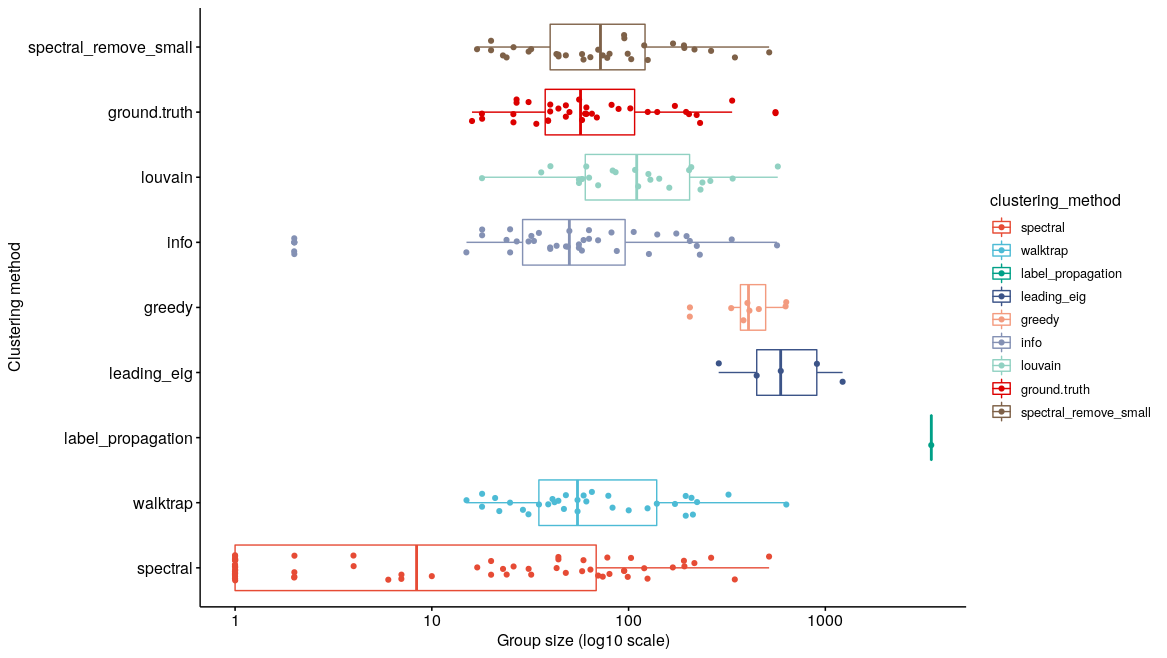
\includegraphics[width=\textwidth]{images/Rplot_draft_plot_boxplot_group_sizes_lfr.png}
      \caption{Boxplot of sizes of communities detected for various clustering methods on a 3457 node 40617 edge benchmark LFR benchmark graph. Code to generate at \url{source('~/RProjects/python_benchmarks/R/plot_boxplot_group_sizes_lfr.R')}}
      \label{fig:boxplot group size lfr clustering methods}
  \end{figure}
 
 
 
  \begin{figure}
      \centering
      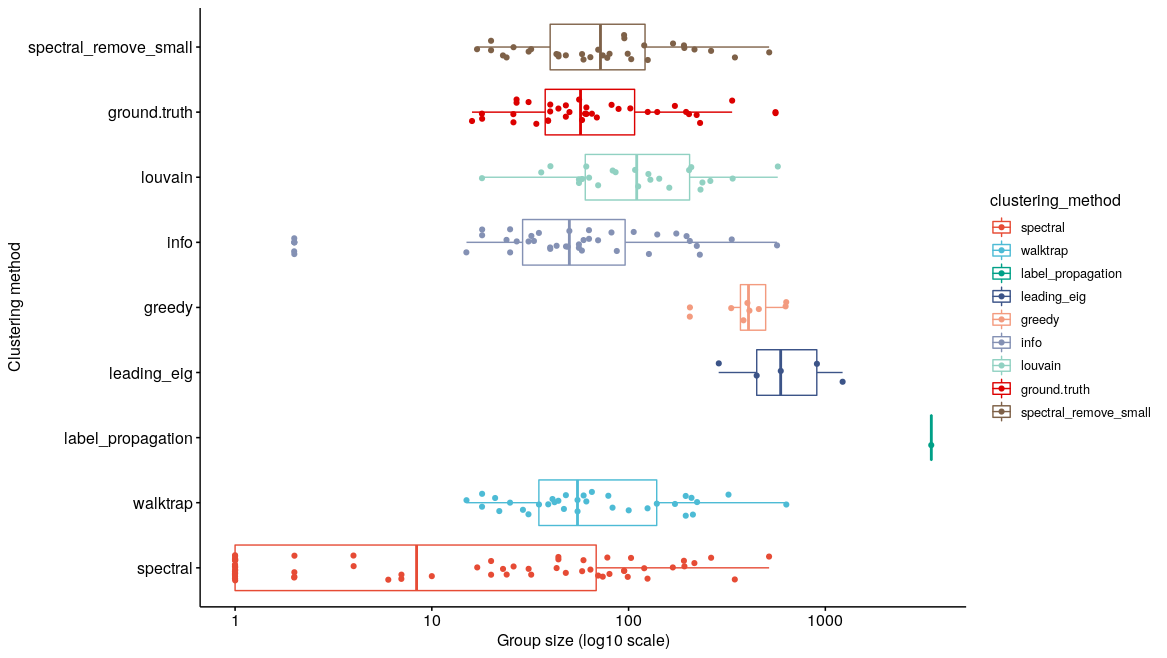
\includegraphics[width=\textwidth]{images/Rplot_draft_plot_boxplot_group_sizes_lfr.png}
      \caption{Boxplot of sizes of communities detected for various clustering methods on a 3457 node 40617 edge benchmark LFR benchmark graph. Code to generate at \url{source('~/RProjects/python_benchmarks/R/plot_boxplot_group_sizes_lfr.R')}}
      \label{fig:boxplot group size lfr clustering methods}
  \end{figure}
 
 
  \begin{figure}
      \centering
          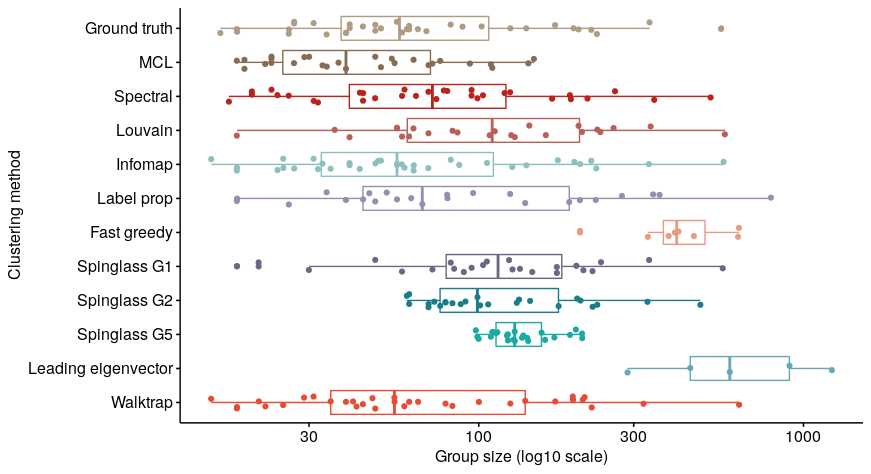
\includegraphics[width=\textwidth]{images/chapter_community_detection/ggplot2/LFR/Rplot_groupsize_filter.png}
      \caption{Boxplot of sizes of communities detected for various clustering methods on a 3457 node 40617 edge benchmark LFR benchmark graph. Code to generate at \url{source('~/RProjects/python_benchmarks/R/plot_boxplot_group_sizes_lfr.R')}}
      \label{fig:boxplot group size lfr clustering methods}
  \end{figure}
  
  
  \subsection{PSP barplots}
  
\begin{figure}
    \centering
    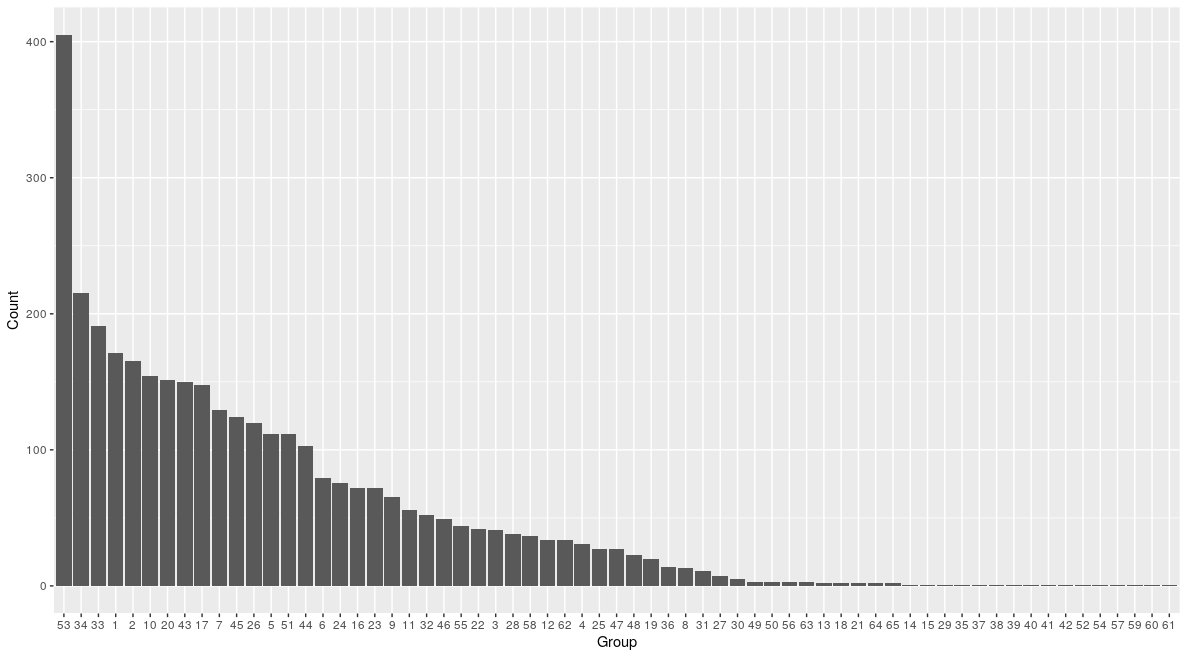
\includegraphics[width=\textwidth]{images/Rplot_group_size_spectral.png}
    \caption{Distribution of group sizes spectral clustering}
    \label{fig:group sizes spectral clustering shows power law distribution}
\end{figure}


\begin{figure}
    \centering
    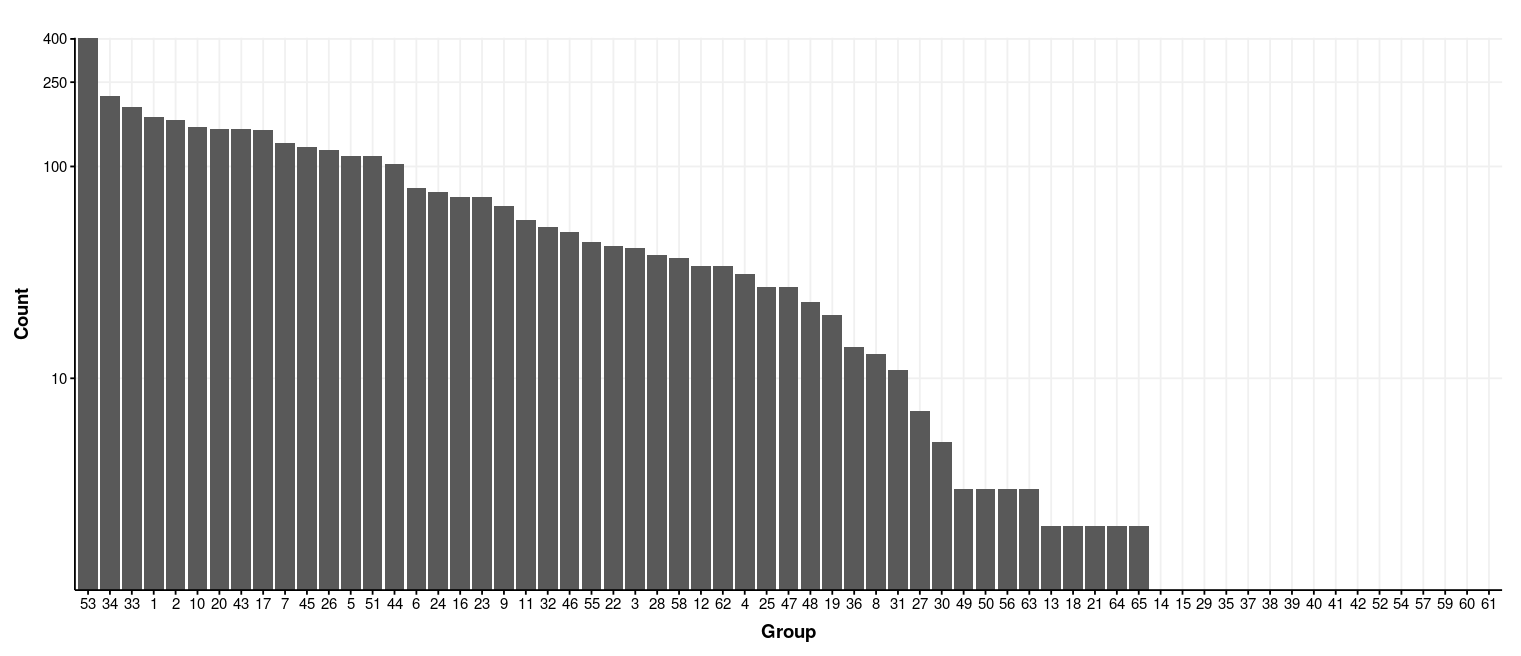
\includegraphics[width=\textwidth]{images/chapter_community_detection/ggplot2/group_size/Rplot_log10_spectral.png}
    \caption{Distribution of group sizes spectral clustering. Log 10 scaled y axis}
    \label{fig:group sizes spectral clustering log 10}
\end{figure}
% latex table generated in R 3.6.3 by xtable 1.8-4 package
% Wed Apr  8 11:31:09 2020

\subsection{Removed SBM}
The stochastic block model performs better when it has more groups rather than when it is nested (SBM level 0 adj NMI 0.846 Communities $n$=52 see also table~\ref{tab:Group sizes compared with ground truth LFR 3457 PSP like benchmark}). The unnested stochastic block model was a has a low modularity partition (Q=0.175) despite good performance on the NMI the converse of fast greedy.


The stochastic block model performs better when it has more groups rather than when it is nested (SBM level 0 adj NMI 0.846 Communities $n$=52 see also table~\ref{tab:Group sizes compared with ground truth LFR 3457 PSP like benchmark}). The unnested stochastic block model was a has a low modularity partition (Q=0.175) despite good performance on the NMI the converse of fast greedy.
% %  Length info = 143
 
% %  Length greedy = 61
 
% %  Length eig = 60
 The stochastic block model performs better when it has more groups rather than when it is nested (SBM level 0 adj NMI 0.846 Communities $n$=52 see also table~\ref{tab:Group sizes compared with ground truth LFR 3457 PSP like benchmark}). The unnested stochastic block model was a has a low modularity partition (Q=0.175) despite good performance on the NMI the converse of fast greedy.
\begin{table}[ht]
\centering
\setlength{\extrarowheight}{2pt}
\begin{tabular}{llllllll}
  \toprule
 & n & Min. & 1Q & Median & Mean & 3Q & Max. \\ 
  \midrule
Ground truth & 36 & 16 & 37.75 & 57.0 & 96.0 & 107.75 & 558 \\ 
Markov Cluster & 1621 & 1 & 1.00 & 1.0 & 2.1 & 1.00 & 148 \\ 
Spectral & 66 & 1 & 1.00 & 8.5 & 52.4 & 68.50 & 518 \\ 
 Louvain & 24 & 18 & 60.25 & 110.0 & 144.0 & 204.25 & 573 \\ 
 Infomap & 39 & 2 & 29.00 & 50.0 & 88.6 & 96.50 & 568 \\ 
 Label Prop. & 26 & 12 & 40.25 & 64.5 & 133.0 & 177.25 & 793 \\ 
 Fast greedy & 8 & 205 & 371.00 & 407.0 & 432.1 & 502.25 & 633 \\ 
 Spinglass gamma1 & 24 & 18 & 79.50 & 115.0 & 144.0 & 180.50 & 564 \\ 
 Spinglass gamma2 & 25 & 60 & 76.00 & 99.0 & 138.3 & 176.00 & 481 \\ 
 Spinglass gamma5 & 25 & 98 & 113.00 & 129.0 & 138.3 & 156.00 & 208 \\ 
 SBM 0 & 52 & 12 & 24.00 & 40.5 & 66.5 & 72.00 & 377 \\ 
 SBM 1 & 10 & 83 & 132.25 & 216.5 & 345.7 & 414.50 & 991 \\ 
 SBM 2 & 3 & 629 & 849.50 & 1070.0 & 1152.3 & 1414.00 & 1758 \\ 
 LEC (Leading eigenvector) & 5 & 287 & 448.00 & 593.0 & 691.4 & 905.00 & 1224 \\ 
 Walktrap & 33 & 15 & 35.00 & 55.0 & 104.8 & 139.00 & 633 \\ 
   \bottomrule
\end{tabular}
\caption{Group sizes compared with ground truth LFR 3457 `PSP like' benchmark. SBM stochastic block model, number refers to level of nesting - level zero is nested in one and in turn nested in two which therefore has the smallest $n=3$ number of communities. 1Q and 3Q first and third quartile. $n$ number of communities} 
\tiny\url{source('~/RProjects/python_benchmarks/R/make_table_gt_lfr_3457.R', echo=TRUE)}
\label{tab:Group sizes compared with ground truth LFR 3457 PSP like benchmark}
\end{table}

\begin{table}[ht]
\centering
\begin{adjustbox}{width=\textwidth}

\setlength{\extrarowheight}{2pt}
\begin{tabular}{rrrrrrrrrrr}
  \toprule
 & Min & 1Q & Median & Mean & 3Q & Max & n & coverage & n comm &  n max comm \\ 
  \midrule
gt & 16 & 37.75 & 57 & 96.03 & 107.75 & 558 & 3457 & 100.00 & 36 & 36 \\ 
  mcl & 18 & 25.00 & 39 & 54.33 & 71.00 & 148 & 1467 & 42.44 & 27 & 1621 \\ 
  spe & 17 & 40.25 & 72 & 105.84 & 121.25 & 518 & 3387 & 97.98 & 32 & 66 \\ 
  louvain & 18 & 60.25 & 110 & 144.04 & 204.25 & 573 & 3457 & 100.00 & 24 & 24 \\ 
  info & 15 & 32.75 & 56 & 95.86 & 111.25 & 568 & 3451 & 99.83 & 36 & 39 \\ 
  label\_prop & 18 & 44.00 & 67 & 137.80 & 190.00 & 793 & 3445 & 99.65 & 25 & 26 \\ 
  fg & 205 & 371.00 & 407 & 432.12 & 502.25 & 633 & 3457 & 100.00 & 8 & 8 \\ 
  SG1 & 18 & 79.50 & 115 & 144.04 & 180.50 & 564 & 3457 & 100.00 & 24 & 24 \\ 
  SG2 & 60 & 76.00 & 99 & 138.28 & 176.00 & 481 & 3457 & 100.00 & 25 & 25 \\ 
  SG5 & 98 & 113.00 & 129 & 138.28 & 156.00 & 208 & 3457 & 100.00 & 25 & 25 \\ 
  sbm0 & 15 & 25.00 & 41 & 67.55 & 75.00 & 377 & 3445 & 99.65 & 51 & 52 \\ 
  sbm1 & 83 & 132.25 & 216 & 345.70 & 414.50 & 991 & 3457 & 100.00 & 10 & 10 \\ 
  sbm2 & 629 & 849.50 & 1070 & 1152.33 & 1414.00 & 1758 & 3457 & 100.00 & 3 & 3 \\ 
  lec & 287 & 448.00 & 593 & 691.40 & 905.00 & 1224 & 3457 & 100.00 & 5 & 5 \\ 
  wt & 15 & 35.00 & 55 & 104.76 & 139.00 & 633 & 3457 & 100.00 & 33 & 33 \\ 
   \bottomrule
\end{tabular}
\end{adjustbox}
\caption{Group sizes compared with ground truth LFR 3457 PSP like benchmark filtered for size less than 15} 
\tiny\url{source('~/RProjects/python_benchmarks/R/make_table_gt_lfr_3457_sizefilter.R')}
\label{tab:Group sizes compared with ground truth LFR 3457 PSP like benchmark filtered for size less than 15}
\end{table}



% latex table generated in R 3.6.3 by xtable 1.8-4 package
% Sun Apr 25 17:53:40 2021
\begin{table}[ht]
\centering
\begin{adjustbox}{width=\textwidth}

\setlength{\extrarowheight}{2pt}
\begin{tabular}{rrrrrrrrrrr}
  \toprule
  & Min & 1Q & Median & Mean & 3Q & Max & n & coverage & n comm &  n max comm \\ 
  \midrule
  gt & 16 & 37.75 & 57 & 96.03 & 107.75 & 558 & 3457 & 100 & 36 & 36 \\ 
mcl & 18 & 25.00 & 39 & 54.33 & 71.00 & 148 & 1467 & 42.44 & 27 & 1621 \\ 
  spe & 17 & 40.25 & 72 & 105.84 & 121.25 & 518 & 3387 & 97.98 & 32 & 66 \\ 
  info & 15 & 32.75 & 56 & 95.86 & 111.25 & 568 & 3451 & 99.83 & 36 & 39 \\ 
  label\_prop & 18 & 44.00 & 67 & 137.80 & 190.00 & 793 & 3445 & 99.65 & 25 & 26 \\ 
  sbm0 & 15 & 25.00 & 41 & 67.55 & 75.00 & 377 & 3445 & 99.65 & 51 & 52 \\ 
   \bottomrule
\end{tabular}
\end{adjustbox}
\caption{Group sizes compared with ground truth LFR 3457 PSP like benchmark filtered for size less than 15} 
\tiny\url{source('~/RProjects/python_benchmarks/R/make_table_gt_lfr_3457_sizefilter2.R')}
\label{tab:Group sizes compared with ground truth LFR 3457 PSP like benchmark filtered for size less than 15 filter}
\end{table}




\subsubsection{Method for LFR benchmark}

\begin{enumerate}
    \item Generate network with degree distribution
    \item Define $\mu$
    \item Generate community size distribution
    \item Each node randomly to a community WHILE community not full
    \item Rewire to keep degree constant but in out degree to satisfy $\mu$
\end{enumerate}
\subsection{Gene Based Statistics}
\textcolor{red}{See chapter xx}

\subsection{results LFR}
\begin{table}[]
    \centering
    \begin{tabular}{lll}
    \toprule
    Comparison with ground truth LFR & NMI  & number of communities \\
    \midrule
    Ground truth & 1 & 36check \\
       louvain  &0.913 & 35\\
 infomap  &0.974 & 23\\
 greedy  &0.564 & 7 check FG NMI although different edges \\ 
 igraph eigenvector& 0.190 & 4 \\
\textbf{ label propagation } & 0.0 & 0\\
 walk trap  & 0.893 & 32\\
 Spectral CDM & 0.782 & 65\\
 \bottomrule
  
    \end{tabular}
    \caption{Performance on lfr 3457 \url{g1 = nx.generators.LFR_benchmark_graph(n=graph_n,tau1= 2.51,tau2 = 1.5,mu= 0.375,average_degree=17,max_degree= 405, min_community= 15,max_community= 1000,seed=seed)} 3457 nodes 39823 edges. See update in file \url{~/Projects_/Python/venvs/Create_LFR_similar_to_PSP-Copy_includeSG.ipynb}}
    \label{tab:Performance on lfr 3457 }
\end{table}

\begin{table}[]
    \centering
    \setlength{\extrarowheight}{2pt}
 \begin{tabular}{ll}
\toprule
Method &  Modularity \\
\midrule
Ground truth        &       0.431 \\
MCL       &       0.127 \\ 
Spectral        &       0.392 \\
Louvain   &       0.432 \\
Infomap    &       0.432 \\
Label prop. &       0.416 \\
Fast greedy         &       0.368 \\
SpinGlass gamma 1        &       0.433 \\
SpinGlass gamma 2       &       0.429 \\
 SpinGlass gamma 5      &       0.380 \\
SBM level 0      &       0.174 \\
SBM level 1       &       0.374 \\
SBM level 2       &       0.259 \\
LEC (igraph eigenvector)        &       0.187 \\
Walk trap         &       0.423 \\
\bottomrule
\end{tabular}
    
    \caption{Modularity of different algorithms partitions for the LFR 3457 40617 graph. The algorithms (for example SpinGlass gamma1, Infomap and Louvain) have found partitions slightly greater than `ground truth'. Ref for Q greater than gt \cite{danon2006effect}. Matches previous now in interesting}
    \tiny\url{g1 = nx.generators.LFR_benchmark_graph(n=graph_n,tau1= 2.51,tau2 = 1.5,mu= 0.375,min_degree=1 (commented out),average_degree=17,max_degree= 405, min_community= 15,max_community= 1000,seed=seed)} seed=1
    \tiny Red machine
    \tiny\url{/home/grant/Projects_/Python/src/get_modularity_lfr.ipynb}
    \label{tab:modularity for the LFR 3457 40617 graph}
\end{table}

I have no explanation for the difference in degree correlation from that reported\cite{orman2009comparison} and further investigation is beyond the scope of this thesis
\subsubsection{Redo}

The performance on the lft benchmark with parameters set as \url{g1 = nx.generators.LFR_benchmark_graph(n=graph_n,tau1= 2.51,tau2 = 1.5,mu= 0.375,average_degree=17,max_degree= 405, min_community= 15,max_community= 1000,seed=seed)} is shown in table~\ref{tab:Performance on lfr 3457 }. Results in a network with 3457 nodes and 39823 edges which was the best approximation I could make using gradual change of the parameters. 

Comparisons of number of communities and summary statistics for community size are shown in table~\ref{tab:Group sizes compared with ground truth LFR 3457 PSP like benchmark}.





\subsection{This is the LFR 3457 with equalish V and E}

subsubsection{bits from removed bit above}
\label{sec:NMI communities}
\todo{method for calculate nmi using python igraph}
But infomap has lower modularity for the network see table~\ref{tab:modularity}


The ground truth modularity for 3457\footnote{\url{g2= nx.generators.LFR_benchmark_graph(n=graph_n, tau1=3, tau2=1.1, mu=0.1, average_degree=10, max_degree=50, min_community=10,max_community=50, seed=1)}} is 0.802 and 0.776 for markov 
\footnote{
\url{/home/grant/Projects_/Python/venvs/benchmark_markov.ipynb}
on red bionic beaver machine.  gml for this at 
}

\url{home/grant/Projects_/Python/venvs/out_graphs/lfr_3457_from_benchmark_markov_clustering.gml}
So it seems like markov and infomap do very well when they are looking for a high modularity but do less well (and find a lower modularity) in our network. Part of the reason may be core periphery structure
\subsubsection{Default setting LFR}
\textbf{default settings }for LFR from Lancichinetti 2012 \cite{lancichinetti2012consensus}

average degree $<k>$= 20, maximum degree kmax = 50, minimum community size cmin = 10, maximum community size cmax = 50, the degree exponent is $\tau1$ = 2, the community size exponent is $\tau2$= 3. This graph is clearly quite different from the PSP. In particular the maximum degree is not far from from average degree (2.5 times average degree)

142 ground truth communities, markov clustering 142

NMI (explain NMI) compare communities 3457 ground truth and markov clustering 0.98858023049201


\begin{table}
\centering
\begin{tabular}{lr}
\toprule
{} &  Adjusted NMI \\
\midrule
info              &         0.971 \\
sg2               &         0.887 \\
sg1               &         0.882 \\
Louvain           &         0.870 \\
wt                &         0.870 \\
sbm level 0       &         0.846 \\
Label prop        &         0.800 \\
sg5               &         0.796 \\
Spectral          &         0.762 \\
sbm level 1       &         0.607 \\
fg                &         0.457 \\
sbm level 2       &         0.307 \\
Markov clustering &         0.295 \\
lec               &         0.134 \\
\bottomrule
\end{tabular}
\caption{Adjusted NMI versus ground truth for V:3457 E:40617 LFR benchmark. Ref adjusted NMI\cite{vinh2010information}}
\tiny\url{/home/grant/Projects_/Python/src/LFR_networkx_to_igraph.ipynb}
\tiny\url{github ipynotebooks_phd.git}
\label{tab:adjusted nmi versus ground truth for 3457 40617 LFR benchmark}
\end{table}


As shown in table~\ref{tab:Group sizes compared with ground truth LFR 3457 PSP like benchmark filtered for size less than 15 filter} the spectral algorithm with fine tuning step as a divisive algorithm has a large number of small communities but these are small and if one considers only those smaller than the default for GSEA (15) 98.0\% of genes are included and the mean and median community size are close to the ground truth. 


The takeaway is in a benchmark where there are no communities of size 1 spectral clustering gives you some but still gives you a reasonable modularity. Infomap despite its good performance gives you 2. 


In a real world network where there are an unknown number of communities spectral gives you 65, 35 of which have more than 15 members. Infomap gives you one massive group and several others of size 1 which is kind of the opposite of what you would like to get but means that info does well on benchmarks and that the spectral one does worse but ok where it counts. 

The number of spectral communities of membership more than 15 is 32. The gready and leading eigenvector method produce numbers of communities noticably different from the ground truth. The spectral methods results are more similar still to ground truth if you consider the distribution of only those groups of size $>$ 15    Min. 1st Qu.  Median    Mean 3rd Qu.    Max. 
 
\subsection{Walk trap results group}
\label{sec:walk trap results}
Implemented in igraph. 562 communities , 405 have single member  Min.1 1st Qu.  1 Median1    Mean 6.151 3rd Qu. 2   Max. 760 

\subsection{Label propagation}

With 10,000 iterations however and keeping the highest modularity division the maximum modularity (on the PSP graph) was 0.256\footnote{0.25565433088497774} after 1 min 28 seconds. After 100,000 iterations the maximum modularity is 0.258\footnote{0.25762367434321437} with a running time of 12m 56 seconds and divided it into 4 communities

Counter(0: 2002, 1: 1404, 2: 37, 3: 2, 4: 12)


\begin{table}[]
    \centering
    \begin{tabular}{llllll}
      Min. &1st Qu.&  Median    &Mean &3rd Qu. &   Max.    \\
       17.00&  40.25&   72.00 & 105.84 &  121.25 & 518.00 .\\
         
    \end{tabular}
    \caption{Spectral groups with members less than fifteen removed}
    \label{tab:my_label}
\end{table}  

\section{To remove}
\subsection{Optimal community size}
\label{sec:optimal community size}
Real world communities tend to show a core and whisker structure. The whiskers tend to be good communities but larger groups discovered by clustering algorithms tend to belong to the core or represent the core and have lower conductance and hence are less cohesive as groups. We can see this pattern of size distribution in the communities discovered in the PSP for particular algorithms \todo{cross ref}.

Approximately 80\% of nodes are in the core \todo{check ref that is from zhukov}
\todo{what does core represent if we are not including core chapter}

\cite{leskovec2010empirical}
\subsection{Paper bits removed}
We calculated gene based statistics for each study using MAGMA (v1.06) using the NCBI 37.3 assembly to identify gene boundaries. \cite{de2015magma}   No window was used around the gene boundaries. Linkage disequilibrium was corrected for using 1000 Genomes European data provided by the CTG lab with the MAGMA software version 1.6.\cite{de2015magma}  Commands used for gene based tests are found in the shell script in supplementary material. Data for the meta-analysis of intelligence performed by Sniekers  et al. was downloaded from the CTG website (see urls). \cite{sniekers2017genome}  The summary statistics for the EA2 study of educational attainment were obtained from the authors and excludes UKBiobank Phase II Education data (used as the discovery cohort) in addition to the data from 23 and me. \cite{okbay2016genome}  The summary statistics unsorted by sex were used for analysis. Summary statistics for Phase II of UKBiobank Education cohort and intelligence cohort were obtained from the co-authors directly from the CCACE.[ref]\todo{get ccace ref}

\subsection{MAGMA GSA methods}

\subsection{GSA MAGMA methods}
Results in \url{/Users/grantrobertson/Programs/copy_paperMagma_draft-master/gene_set}

raw output listed in \url{ls gene_set/*PPI_PSD_clean_Published.gmt*} from the directory above geneset

`savage is \url{less gene_set/savage_int_10_PPI_PSD_clean_Published.gmt.sets.out }



\subsubsection{The GSEA software}

The GSEA software is implemented in Java and has a graphical user and command line interface. The input format for gene sets provided by the user is either a gene matrix file ,gmx or a gene matrix transpose file .gmt.
These consist of tab or space separated files headed with the set name and with the gene names along the columns or rows.
 \footnote{MAGMA uses gmt and also gmt is easier if you are using python and building them up by using a number and a hash to a list with the gene elements in in addition gmx is difficult to implement using a dataframe (which is what it looks like it is designed for) because dataframes require the same length.} The Broad Institute suggests using spreadsheet software such as Excel to generate the files (see methods) (see Zeeburg \cite{zeeberg2004mistaken} for errors with excel) and \cite{ziemann2016gene}
 Version Java version Code
\footnote{include ref for the errors due to date}
 \footnote{also note in the intelligence literature ? have people used the full gmx list even although there is a high prior probability that they involve neural tissues what would be the result of the published studies if we only looked at gene terms that are neural USE NIGO set  Geifman et al}



\textcolor{red}{gnomad and cross ref - also add DEG}
The Exome Aggregation Consortium (ExAC - Broad Institute) contains DNA sequence data from the exomes of 60,706 individuals and provides metrics to identify genes subject to strong selection pressure against mutation. \cite{lek2016analysis}  We used data from version 1 (see URLs for source). This provides gene level measures of intolerance to deleterious mutations. The post synaptic density is known to be under evolutionary constraint with a low dN/dS (amino acid change/synonymous mutation change) in both murine and human PSD. \cite{ryan2009origin},\cite{bayes2012comparative},\cite{bayes2011characterization}  A bi-map was made between Ensembl transcript id in the ExAC data download and Entrez-id for the GRCh37 assembly using BioMart. \cite{smedley2015biomart}  We used the probability of the loss of function intolerance (pLI) to measure genetic constraint.

\todo{low conductance and high conductance nodes. perhaps high vanish and you have a plum pudding model}


\subsubsection{Gene level results}

Genome wide gene association analysis (GWGAS) was performed with MAGMA using the summary statistical data from the four cohorts. The results, including MAGMA output files, are available in the Supplemental Information.
Sniekers et al. found 47 genes associated with intelligence using MAGMA (Bonferroni threshold of P = $2.73 x 10^{-6}$). \cite{sniekers2017genome}  To confirm the validity of our gene level results we used summary data provided from this study and found 46 genes at  P$<2.74 x 10^{-6}$ genes using MAGMA v.1.06.  The pairwise correlation (Spearman’s $\rho$) of the negative log10 transformed gene p values reported in the supplementary material found in Sniekers et al and our results was $\rho$= 0.957\cite{sniekers2017genome} (cross ref). 



 \section{Enrichment of the presynaptic proteome}
 
 Surprisingly all of the education phenotypes enrich for genes in the presynaptic proteome and this is not true of intelligence except weakly for UKBB Intelligence Discovery. The reasons for this are unclear. See figure \ref{Table:Enrichment of intelligence phenotypes presynaptic proteome} and \ref{Table:Enrichment of education phenotypes presynaptic proteome}
 


\begin{table}
\centering
\begin{tabular}{rlrrrrr}
  \hline
 & SET & NGENES & BETA & BETA\_STD & SE & P \\ 
  \hline
1 & Education Replication\_presynaptic\_all & 1449 & 0.06 & 0.02 & 0.02 & 0.0048 \\ 
  2 & Education Discovery\_presynaptic\_all & 1461 & 0.07 & 0.02 & 0.03 & 0.0032 \\ 
  3 & EA3\_presynaptic\_all & 1460 & 0.10 & 0.03 & 0.03 & 0.0020 \\ 
   \hline
\end{tabular}
\caption{Enrichment of education phenotypes presynaptic proteome} 
\label{Table:Enrichment of education phenotypes presynaptic proteome}
\end{table}




% latex table generated in R 3.6.1 by xtable 1.8-4 package
% Thu Jan 16 16:01:27 2020
\begin{table}[ht]
\centering
\begin{tabular}{rlrrrrr}
  \hline
 & SET & NGENES & BETA & BETA\_STD & SE & P \\ 
  \hline 

1 & Intelligence Discovery\_presynaptic\_all & 1461 & 0.05 & 0.01 & 0.03 & 0.04 \\ 
  2 & Intelligence Replication\_presynaptic\_all & 1466 & 0.02 & 0.00 & 0.02 & 0.23 \\ 
  3 & Savage\_presynaptic\_all & 1498 & 0.04 & 0.01 & 0.03 & 0.10 % latex table generated in R 3.6.3 by xtable 1.8-4 package
% Sat Apr 24 13:35:54 2021
\begin{table}[ht]
\centering
\begin{tabular}{llrrrr}
  \toprule
ID & Name & n & n in PSP & p & q FDR B.H \\ 
  \midrule
GO:0030165 & PDZ domain binding & 26 & 58 & $6.01 \times 10^{-21}$ & $2.75 \times 10^{-18}$ \\ 
  GO:0022803 & passive transmembrane transporter activi & 40 & 179 & $5.70 \times 10^{-19}$ & $8.70 \times 10^{-17}$ \\ 
  GO:0015267 & channel activity & 40 & 179 & $5.70 \times 10^{-19}$ & $8.70 \times 10^{-17}$ \\ 
  GO:0038023 & signaling receptor activity & 33 & 136 & $8.38 \times 10^{-17}$ & $7.67 \times 10^{-15}$ \\ 
  GO:0060089 & molecular transducer activity & 33 & 136 & $8.38 \times 10^{-17}$ & $7.67 \times 10^{-15}$ \\ 
  GO:0008066 & glutamate receptor activity & 15 & 21 & $1.20 \times 10^{-16}$ & $9.14 \times 10^{-15}$ \\ 
  GO:0022857 & transmembrane transporter activity & 47 & 292 & $3.49 \times 10^{-16}$ & $2.24 \times 10^{-14}$ \\ 
  GO:0046873 & metal ion transmembrane transporter acti & 34 & 152 & $3.97 \times 10^{-16}$ & $2.24 \times 10^{-14}$ \\ 
  GO:0022836 & gated channel activity & 28 & 100 & $4.40 \times 10^{-16}$ & $2.24 \times 10^{-14}$ \\ 
  GO:0005216 & ion channel activity & 35 & 163 & $5.33 \times 10^{-16}$ & $2.44 \times 10^{-14}$ \\ 
   \bottomrule
\end{tabular}
\caption{Group 7 GO: Molecular Function 91 significant terms} 
\label{tab:Group 7 GO: Molecular Function 91 significant terms}
\end{table}\\ 
  4 & Davies\_presynaptic\_all & 1460 & 0.05 & 0.01 & 0.03 & 0.04 \\ 
   \hline
\end{tabular}
\caption{Enrichment of intelligence phenotypes presynaptic proteome \url{'~/RProjects/paper_xls_output/R/make_pLI_correlation}...., line 507} 
\label{Table:Enrichment of intelligence phenotypes presynaptic proteome}
\end{table}

Those of low betweeness are a slightly smaller group but enrich more in ea2 and ukbbed. Todo correlation of graph degree etc and study in presynaptic. \url{source('~/RProjects/graph_distances/R/collate_presynaptic_edubet.R')}
 

The most enriched genes in toppgene are labelled as post synaptic including BSN, SHANK3 and CAMKV. There is overlap between presynaptic and PSP (\todo{how much overlap}) A large number of the highest scoring presynaptic genes are listed as post synaptic in toppgene. \todo{MAGMA GSA for toppgene presynaptic genes}





\section{Unused tables}

% latex table generated in R 3.6.3 by xtable 1.8-4 package
% Wed Apr  7 18:34:17 2021
\begin{table}[ht]
\centering
\setlength{\extrarowheight}{2pt}
\begin{tabular}{llllrrrrrr}
  \toprule
PSP & group5 & glutamate & g-protein & mean & median & IQR & min & nax & n \\ 
  \midrule
True   & True   & True   & False   & 0.751 & 0.999 & 0.249 & 1.195E-09 & 1 & 8 \\ 
  True   & False   & True   & False   & 0.761 & 0.997 & 0.282 & 2.305E-07 & 1 & 14 \\ 
  True   & False   & True   & True   & 0.746 & 0.955 & 0.277 & 9.392E-03 & 1 & 12 \\ 
  True   & True   & True   & True   & 0.654 & 0.889 & 0.859 & 2.236E-13 & 1 & 9 \\ 
  True   & False   & False   & True   & 0.551 & 0.759 & 0.998 & 1.861E-164 & 1 & 139 \\ 
  True   & True   & False   & False   & 0.514 & 0.679 & 0.984 & 2.704E-26 & 1 & 66 \\ 
  True   & True   & False   & True   & 0.477 & 0.506 & 0.909 & 1.125E-14 & 1 & 29 \\ 
  False   & False   & True   & False   & 0.419 & 0.374 & 0.852 & 1.333E-07 & 1 & 10 \\ 
  True   & False   & False   & False   & 0.437 & 0.197 & 0.986 & 8.411E-70 & 1 & 3130 \\ 
  False   & False   & False   & True   & 0.130 & 0.002 & 0.074 & 3.174E-39 & 1 & 1009 \\ 
  False   & False   & False   & False   & 0.210 & 0.001 & 0.255 & 8.222E-118 & 1 & 13946 \\ 
  False   & False   & True   & True   & 0.336 & 0.000 & 0.678 & 1.601E-42 & 1 & 7 \\ 
   \bottomrule
\end{tabular}
\caption{Probability of loss of function intolerance for PSP, group 5 and glutamate\textcolor{red}{not sure min max ads much you could say max 1 and min varies from x to y Min 1.861E-164 to 9.392e-03}} 
\tiny\url{source('~/RProjects/chapter_community_detection/R/group5/pLI/summarise_pLI.R')}
\label{tab:Probability of loss of function intolerance for PSP, group 5 and glutamate}
\end{table}
\todo{discussion removed here}
\textcolor{red}{discussion removed here}
 
 % latex table generated in R 3.6.3 by xtable 1.8-4 package
% Wed Apr  7 18:42:03 2021
\begin{table}[ht]
\centering
\begin{tabular}{lllrrrrrr}
  \toprule
PSP & group5 & glutamate & mean & median & IQR & min & nax & n \\ 
  \midrule
True   & FALSE & TRUE & 0.754 & 0.985 & 0.286 & 2.305E-07 & 1 & 26 \\ 
  TRUE & TRUE & TRUE & 0.699 & 0.983 & 0.874 & 2.236E-13 & 1 & 17 \\ 
  TRUE & TRUE & FALSE & 0.503 & 0.542 & 0.958 & 2.704E-26 & 1 & 95 \\ 
  FALSE & FALSE & TRUE & 0.384 & 0.363 & 0.747 & 1.601E-42 & 1 & 17 \\ 
  TRUE & FALSE & FALSE & 0.441 & 0.216 & 0.987 & 1.861E-164 & 1 & 3269 \\ 
  FALSE & FALSE & FALSE & 0.204 & 0.001 & 0.230 & 8.222E-118 & 1 & 14955 \\ 
   \bottomrule
\end{tabular}
\caption{Probability of loss of function intolerance for PSP, group 5 and glutamate. Median for glutamate and gprotein removed group5 is 0.679} 
\label{tab:Probability of loss of function intolerance for PSP, group 5 and glutamate}
\end{table}





\begin{table}[ht]
\centering
\setlength{\extrarowheight}{2pt}
\begin{tabular}{llllllll}
  \toprule
PSP & group5 & glutamate & g protein & mean & median & IQR & $n$ \\ 
  \midrule
True   & True   & True   & False & 0.751 & 0.999 & 0.249 & 8 \\ 
  True   & False & True   & False & 0.761 & 0.997 & 0.282 & 14 \\ 
  True   & False & True   & True   & 0.746 & 0.955 & 0.277 & 12 \\ 
  True   & True   & True   & True   & 0.654 & 0.889 & 0.859 & 9 \\ 
  True   & False & False & True   & 0.551 & 0.759 & 0.998 & 139 \\ 
  True   & True   & False & False & 0.514 & 0.679 & 0.984 & 66 \\ 
  True   & True   & False & True   & 0.477 & 0.506 & 0.909 & 29 \\ 
  False & False & True   & False & 0.419 & 0.374 & 0.852 & 10 \\ 
  True   & False & False & False & 0.437 & 0.197 & 0.986 & 3130 \\ 
  False & False & False & True   & 0.130 & 0.002 & 0.074 & 1009 \\ 
  False & False & False & False & 0.210 & 0.001 & 0.255 & 13946 \\ 
  False & False & True   & True & 0.336 & 0.000 & 0.678 & 7* \\ 
   \bottomrule
\end{tabular}
\caption{Probability of loss of function intolerance for PSP, group 5 and glutamate. Minumum and maximum values not shown. Minimum ranges $1.68 \times 10^{-164}$ to $9.32\times 10^{-3}$. Maximum pLI is one for all groups. Not there is overlap between GO0007215:glutamate receptor signalling pathway and GO0007186:Gprotein coupled biological process} 
\tiny\url{source('~/RProjects/chapter_community_detection/R/group5/pLI/summarise_pLI.R')}
\label{tab:Probability of loss of function intolerance for PSP, group 5 and glutamate}
\end{table}

% latex table generated in R 3.6.3 by xtable 1.8-4 package
% Thu Apr  8 17:56:55 2021

\subsection{Overlap with other partitions}

Group 5 Spectral was distributed quite widely but there were 31 in group 16, 10 in 21 and 19 in 24 using infomap. Group 24 is enriched in the savage study and contains GRIP1, GRIA 1-4, GRIK 1,2,3,5, 3 metabotropic, PICK1, GRIP AP and CACNG2. This seems to be a cohesive group across different clusterings (see below) code \url{source('~/RProjects/graph2community/R/overlap_info.R')}

\todo{take 1 neighbourhood of these genes}

For the overlap between group 5 
and louvain group 7 22 were in group 7 and 57 in Louvain 14.

The 22 gene overlap between group 5 and louvain group 7 were ampa, kainate and 3 metabotropic glutamate along with PICK1 and GRIP AP1 and a few others. GSA 13 glutamate receptor activity GO:0008066 

This supports the Newman idea that different partitions are made up of similar components. 

\todo{can add that infomap and Louvain along with spectral are the ones most recommended by Newman and that group has expertise with spectral also to add and look at overlap for block stochastic.}


\subsection{NMI and group size}
 How NMI varies with group size and ground truth. Usefulness of LFR benchmark. Didn't use the Newman one as fairly straightforward. Didn't use the SNAP databases because of the issue of ground truth and it was just something I didn't get round to doing but it would be a reasonable thing for further work. 
 You could look at the combination of features that are best for a clustering algorithm using k means clustering like that paper on stats methods for GSA \url{https://bmcbioinformatics.biomedcentral.com/articles/10.1186/s12859-017-1674-0}
 
 

\section{tmpout}

 It is interesting to note that one of the only findings within this group is an enrichment for neurogenesis. GSA enrichment for neurogenesis has been reported in a large GWA study of intelligence\cite{hill2019combined} but that gene set was over 1000 genes in size, this group, by contrast is 7 genes and enriches. 




The general changing of tools led to the abandonment of DisGen




  \subsection{SNPs outside gene and WGS}
 
 Not using leaf structure of GO. 
 
 Lack of drop in clipped ontology and clipped disease ontology (section 4)
\section{Chapter 3}
\subsection{Omnigenic}


\todo{add naomi wray article}.

at such When moving from a trait such as intelligence to polygenic disorders that have different onsets in time then if we assume these to be synaptopathies we can expect different proteins to be expressed and this to correspond to the critical periods of the emergence of the disorder. For example neurodevelopmental disorders early, schizophrenia we would expect to occur around the time of peak onset of schizophrenia.




Group 5 and 20 with pascal 


Data over timespan from \url{http://www.brainspan.org/} cited by Okbay and used 

Future analyses may also be able to incorporate data on gene expression

and also things like eqtl, chromatin states and epigenomics. Also as well as time course to look at brain areas. 

Surprisingly non random things make probabilistic models difficult


 A final potential issue is that many studies that use gene ontology terms use them as a list ignoring the connections between them and the propagation from leaf to root that takes place in dedicated ontology enrichment analyses \cite{rhee2008use}\cite{mi2019protocol} \footnote{compare with several cognitive GSA inc Hill and Sneikers that use these as part of a list with reactome terms and msig}
 Depict
Takeaway - something under recent active development flexible ie will take as its input our gene set which is why we dont use depict because the big thing about depict is you give us your snp values from your GWAS and we do everything under the sun with it and highlight lots of potential pathways wheras what we want is to say we want to check this list of genes with this study 

 \subsection{Clustering using metadata as described by Newman}
 This is really the joint thing you were talking about earlier 
 \subsection{Genetic constraint}
 Previous DH paper. Genetic constraint really high in PSP. I cannot help but think that this is in some way ameliorated by the gene reduplication event and network architecture will reflect this development. The use of pLI provides evidence of the effects of network centrality on genetic constraint in humans.



Data freezing
 Version control 
 Some things are interesting but don't work computationally as complexity increases eg VEGAS, the Newman python code for the message passing algorithm, Newman and Girvan model. 
 Availability of data for benchmarking eg MAGMA for published papers. 
 
 I would suggest that package developers produce a dataset even synthetic data and have these are the results you would expect to get if you ran everything right. A synthetic benchmark could also help comparison with MAGMA and PASCAL for example. 
 
  \subsection{Study design SG to discussion}
We would however prefer not to abandon spin glass entirely. McLean (personal commmunication) found it gave good community enrichment at certain values (higher values) of gamma. However we are also aware both from theory and our earlier experiment that pure modules in the ontology sense may not be what we want. We may want a dominant ontology group and their neighbouring proteins that form a module as this may map more reliably onto population data. Also although it is attractive the ontology group is in no sense a ground truth  (Kronecker).\todo{remove this}



It is interesting to note the flaws with NMI in assessing benchmark performance. This is an example of an area where good practices have been developed but they have not been used in a practical setting. NMI is a very good measure of clustering performance in comparison to \cite{newman2018networks} but it has the drawback that as the number of communities increases NMI increases, using adjusted NMI is a very nice workround but this is an example of one of many small issues that one never considers until doing a practical project. 

\subsection{Power and study design}
 
 A striking feature of the GSA performed on the samples discussed in chapter 2 is the lack of any significant findings with the exception of the use of DEPICT on EA2. Undoubtedly the reason for this is the sheer number of gene sets tested and this is exacerbated by not using the inherent structure in gene ontologies. 
 
 You can afford to throw away signal by doing lots of tests (eg MAGMA GSA) because with intelligence (and especially educational attainment N will get great enough that the signal will out. The findings of the community detection improve with increased N but it was difficult to find a way to limit the number of tests performed in a principled way. For some rarer but by no means rare disorders/symptom complexes (give example of d induced psychosis) one may no achieve such numbers and there are a number of diseases which are common enough but too rare to allow such a wasteful approach at present BPAD for example is in this category although this may change it will not change for all disorders.
 
 
 
Diagnosis, UMLS

 There are examples where redefining the groups contained within a disease group have yielded better correlation with progression and prognosis. 

Importance of tissues specificity from chapter 2 \subsubsection{Value of tissue specific networks}
\label{sec:value_of_tissue_specific_networks}

\cite{parikshak2015systems} quotes the example of cardiac PPI to investigaste long QT in \cite{lundby2014annotation}

Kitsak and Barabasi \cite{kitsak2016tissue}
also regional specificity of network see recent SG work on synaptome maps. 



 often it is not the predominant ontology member in a group that is associated with the phenotype but an agglomeration of supporting proteins which often have little in common other than their close interaction with the ontology members found to be associated with a phenotype in animal studies. In pursuing a very 'pure' functional enrichment using gene ontology for example as ones objective function using methods that have tunable parameters one misses these associated proteins. 

\subsection{Community structure and choice of algorithm}

Although the summation constraint \todo{look up} may avoid the trivial modularity solution (putting all vertices in one module) it does not avoid the 'near trivial' situation such as cone community with 99\% of the nodes and another with 1\%. Pocklington used visual inspection to fine tune the initial clustering but this is difficult when we have large numbers of vertices and is a potential source of bias if we are doing inference for example using population data. Some clustering modalities such as spin glass allow control over the number of communities with the approximate influence of size but there is the problem of tunable paramaters. Other such as Louvain are heirarchical (CDM is too) but often the implementation does not allow access tro the heirarchy or one is back with the problem of choosing the division that looks right (ie the level in the height of the heurarchy) rather than maximising the modularity or likelihood with consequent problems in inference. 

The best pragmatic solution so far may be to choose a method that gives `pretty good` (with the earlier caveat about problems in looking for too pure a functional enrichment)ideally one without tubale parameters. 

In our experience of the synaptic proteome spectral clustering and Louvain perform well although the groups are rather large with Louvain. In the future especially with access to raw genotype data maximising the joint (improbability) of the population study and clustering may be effective ie we accept a small decrease in modularity if it is associated with a partition that makes sense of the study but then there is the question of how small the change in modularity can be. 



We need a way in which we can take into account that the pre and post synaptic areas are integrated eg some processes cross them and form cross synaptic modules and also that some genes are present in both compartments. It seems that the isolated post synaptic component is enriched for educational attainment but a number of the most significant genes are those seen in the PSP.








 

 \subsection{Lessons learned}
 
 I considerably underestimated the complexity of mapping identifier terms both between different systems (Entrez and Ensembl) and between different features (eg Entrez and CUI). A lot of modern web interface software hides this complexity from the user (eg FUMA) but makes reconstructing an analysis more difficult. One also tends to underestimate the complexity of any task one has even partially mastered, the difficulty of translating ids is probably one of the reasons for the continued popularity of the Gene enrichment platform DAVID. 
 
 Visualisation of networks is very useful and there are a number of excellent packages available. I found Gephi to be particularly intuitive for me. There is however an increasing deviation between network size and efficient visualisation. One thing that would have been very helpful would be a way to dynamically view hierarchy or use custom embeddings (for example the first two eigenvectors of the laplacian) or animation (viewing communities as a diffusion process). Gephi remains in my opinion the best visualisation software but I wonder whether highly optimised physics based engines such as Unity may have something to offer and whether visualisations that truly allow three dimensional viewing may be more practicable in the near future. It is likely that those who have the skills to implement these solutions may not be aware of these needs and it is a possible opportunity for cross disciplinary working. 
 
 
 
 
 
 Importance of visualisation software ? some improvements especially with embedding. Gephi very nice ? build on an engine such as unity since most of the models are physics based and the layouts are the things that take computational power.
 

 
 \subsection{Issue of neuropsychiatric diagnosis}
 Disgennet how population studies map to disease terms. Changing DSM. It would be useful if things like Disgennet mapped to clinical codes (eg ICD) 
 
 You have to repeat these studies for each disease before you can reach a conclusion about disease but there are some putative signals from disease term enrichment in ch 3 about core and periphery and key nodes. 
 
 
Study design and increase in GWA size

Small differences in modularity can fice rise to difference ocmmunities. ? jointly optimise.
Did not include motifs or core periphery





Does not take into account also dynamic effects e.g. rules based modelling discuss this briefly and also spatial orientation within the larger synapse (functional organisation of post synaptic glutamate receptors MacGillavry
